\section{Numpy} % (fold)
\label{sec:numpy}

\begin{frame}\frametitle{Numpy}
    \framesubtitle{}

    \begin{itemize}
        \item Fundamental package for scientific computing with Python
        \item N-dimensional array object
        \pause
        \item Linear algebra, Fourier transform, random number capabilities
        \item Building block for other packages (e.g. Scipy)
        \item Open source
    \end{itemize}

\end{frame}

\begin{frame}\frametitle{import numpy as np}
    \framesubtitle{The basics}

    Basics:

    \codeblock{code/numpy_basics.py}

    Slicing as usual.

\end{frame}

\begin{frame}\frametitle{More basics}
    \framesubtitle{}

    \codeblock{code/numpy_basics2.py}

\end{frame}

\begin{frame}\frametitle{More basics}
    \framesubtitle{}

    \codeblock{code/numpy_basics3.py}

\end{frame}

\begin{frame}\frametitle{Arrays are mutable}

    \codeblock{code/numpy_mutable.py}

\end{frame}

\begin{frame}\frametitle{Array attributes}
    \framesubtitle{}

    \codeblock{code/numpy_attr.py}

\end{frame}

\begin{frame}[fragile]\frametitle{Basic operations}
    \framesubtitle{}

    Arithmetic operators: \textbf{elementwise} application

    \codeblock{code/numpy_ops.py}

    Also, we can use \verb|+=| and \verb|*=|.

\end{frame}

\begin{frame}\frametitle{Array broadcasting}
    \framesubtitle{}

    When operating on two arrays, numpy compares shapes.
    Two dimensions are compatible when
    \begin{enumerate}
        \item They are of equal size
        \item One of them is 1
    \end{enumerate}

\end{frame}

\begin{frame}\frametitle{Array broadcasting}
    \framesubtitle{An example}

    \begin{figure}
        \centering
        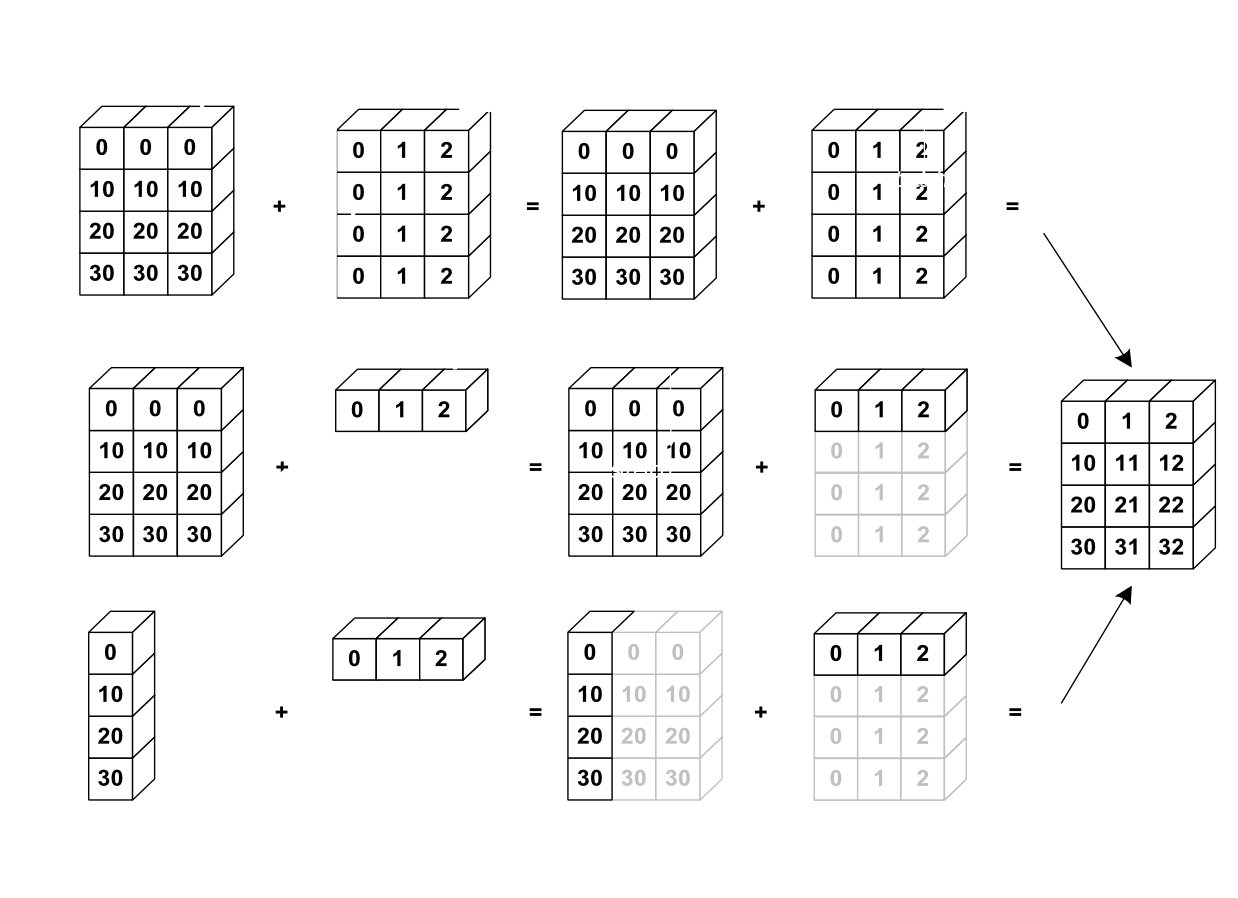
\includegraphics[scale=0.3]{img/broadcasting.png}
    \end{figure}

\end{frame}

\begin{frame}\frametitle{Array broadcasting with scalars}


    This also allows us to add a constant to a matrix or multiply a matrix by a constant


    \codeblock{code/numpy_scalar_ops.py}


\end{frame}

\begin{frame}\frametitle{Vector operations}
    \begin{itemize}
        \item inner product
        \item outer product
        \item dot product (matrix multiplication)
    \end{itemize}

    \codeblock{code/numpy_vector_ops.py}

\end{frame}

\begin{frame}\frametitle{Matrix operations}

    First, define some matrices:

    \codeblock{code/numpy_matrix.py}

\end{frame}

\begin{frame}\frametitle{Matrix operations}

    \codeblock{code/numpy_matrix_ops.py}

\end{frame}



\begin{frame}\frametitle{Operations along axes}
    \framesubtitle{}

    \codeblock{code/numpy_ops2.py}

\end{frame}

\begin{frame}\frametitle{Slicing arrays}
    \framesubtitle{}

    More advanced slicing

    \codeblock{code/numpy_slice.py}

\end{frame}

\begin{frame}\frametitle{Iterating over arrays}
    \framesubtitle{}

    \begin{itemize}
        \item Iterating over multidimensional arrays is done with respect
        to the first axis: \texttt{for row in A}
        \item Looping over all elements:
        \texttt{for element in A.flat}
    \end{itemize}

\end{frame}

\begin{frame}\frametitle{Reshaping}
    \framesubtitle{}

    Reshape using \texttt{reshape}.
    Total size must remain the same.

    \vfill\pause

    Resize using \texttt{resize},
    always works: chopping or appending zeros

    First dimension has `priority', so beware of unexpected results

    \vfill\pause

    Try it!

\end{frame}

\begin{frame}\frametitle{Matrix operations}

\texttt{import numpy.linalg}

\begin{table}
\centering
\begin{tabular}{@{}ll@{}}
    \texttt{eye(3)}& Identity matrix\\
    \texttt{trace(A)}& Trace\\
    \texttt{column\_stack((A,B))}& Stack column wise\\
    \texttt{row\_stack((A,B,A))}& Stack row wise
\end{tabular}
\end{table}

\end{frame}

\begin{frame}[fragile]\frametitle{Linear algebra}
    \framesubtitle{}

\texttt{import numpy.linalg}

\begin{table}
\centering
\begin{tabular}{@{}ll@{}}
    \texttt{qr}& Computes the QR decomposition\\
    \texttt{cholesky}& Computes the Cholesky decomposition\\
    \texttt{inv(A)}& Inverse\\
    \texttt{solve(A,b)}& Solves $Ax = b$ for $A$ full rank\\
    \texttt{lstsq(A,b)}& Solves $\arg\min_x \|Ax-b\|_2$\\
    \texttt{eig(A)}& Eigenvalue decomposition\\
    \texttt{eig(A)}& Eigenvalue decomposition for
    symmetric or hermitian\\
    \texttt{eigvals(A)}& Computes eigenvalues.\\
    \texttt{svd(A, full)}& Singular value decomposition\\
    \texttt{pinv(A)}& Computes pseudo-inverse of A
\end{tabular}
\end{table}
\end{frame}

\begin{frame}\frametitle{Fourier transform}

\texttt{import numpy.fft}

\begin{itemize}
    \item \texttt{fft} 1-dimensional DFT
    \item \texttt{fft2} 2-dimensional DFT
    \item \texttt{fftn} N-dimensional DFT
    \item \texttt{ifft} 1-dimensional inverse DFT (etc.)
    \item \texttt{rfft} Real DFT (1-dim)
    \item \texttt{ifft} Imaginary DFT (1-dim)
\end{itemize}

\end{frame}

\begin{frame}\frametitle{Random sampling}

\texttt{import numpy.random}

\begin{table}
\centering
\begin{tabular}{@{}ll@{}}
    \texttt{rand(d0,d1,...,dn)} & Random values in a given shape\\
    \texttt{randn(d0, d1, ...,dn)} & Random standard normal\\
    \texttt{randint(lo, hi, size)} & Random integers [lo, hi)\\
    \texttt{choice(a, size, repl, p)} & Sample from a\\
    \texttt{shuffle(a)} & Permutation (in-place)\\
    \texttt{permutation(a)} & Permutation (new array)
\end{tabular}
\end{table}

\end{frame}

\begin{frame}\frametitle{Distributions in random}
\texttt{import numpy.random}

    The list of distributions to sample from is quite long, and includes
\begin{itemize}
    \item \texttt{beta}
    \item  \texttt{binomial}
    \item \texttt{chisquare}
    \item \texttt{exponential}
    \item \texttt{dirichlet}
    \item \texttt{gamma}
    \item \texttt{laplace}
    \item \texttt{lognormal}
    \item \texttt{pareto}
    \item \texttt{poisson}
    \item \texttt{power}
\end{itemize}


\end{frame}

% section numpy (end)
